\chapter{Supplementary Figures}
\label{cp:02-Figures-SI}

\begin{figure}[!htpb]
    \centering
    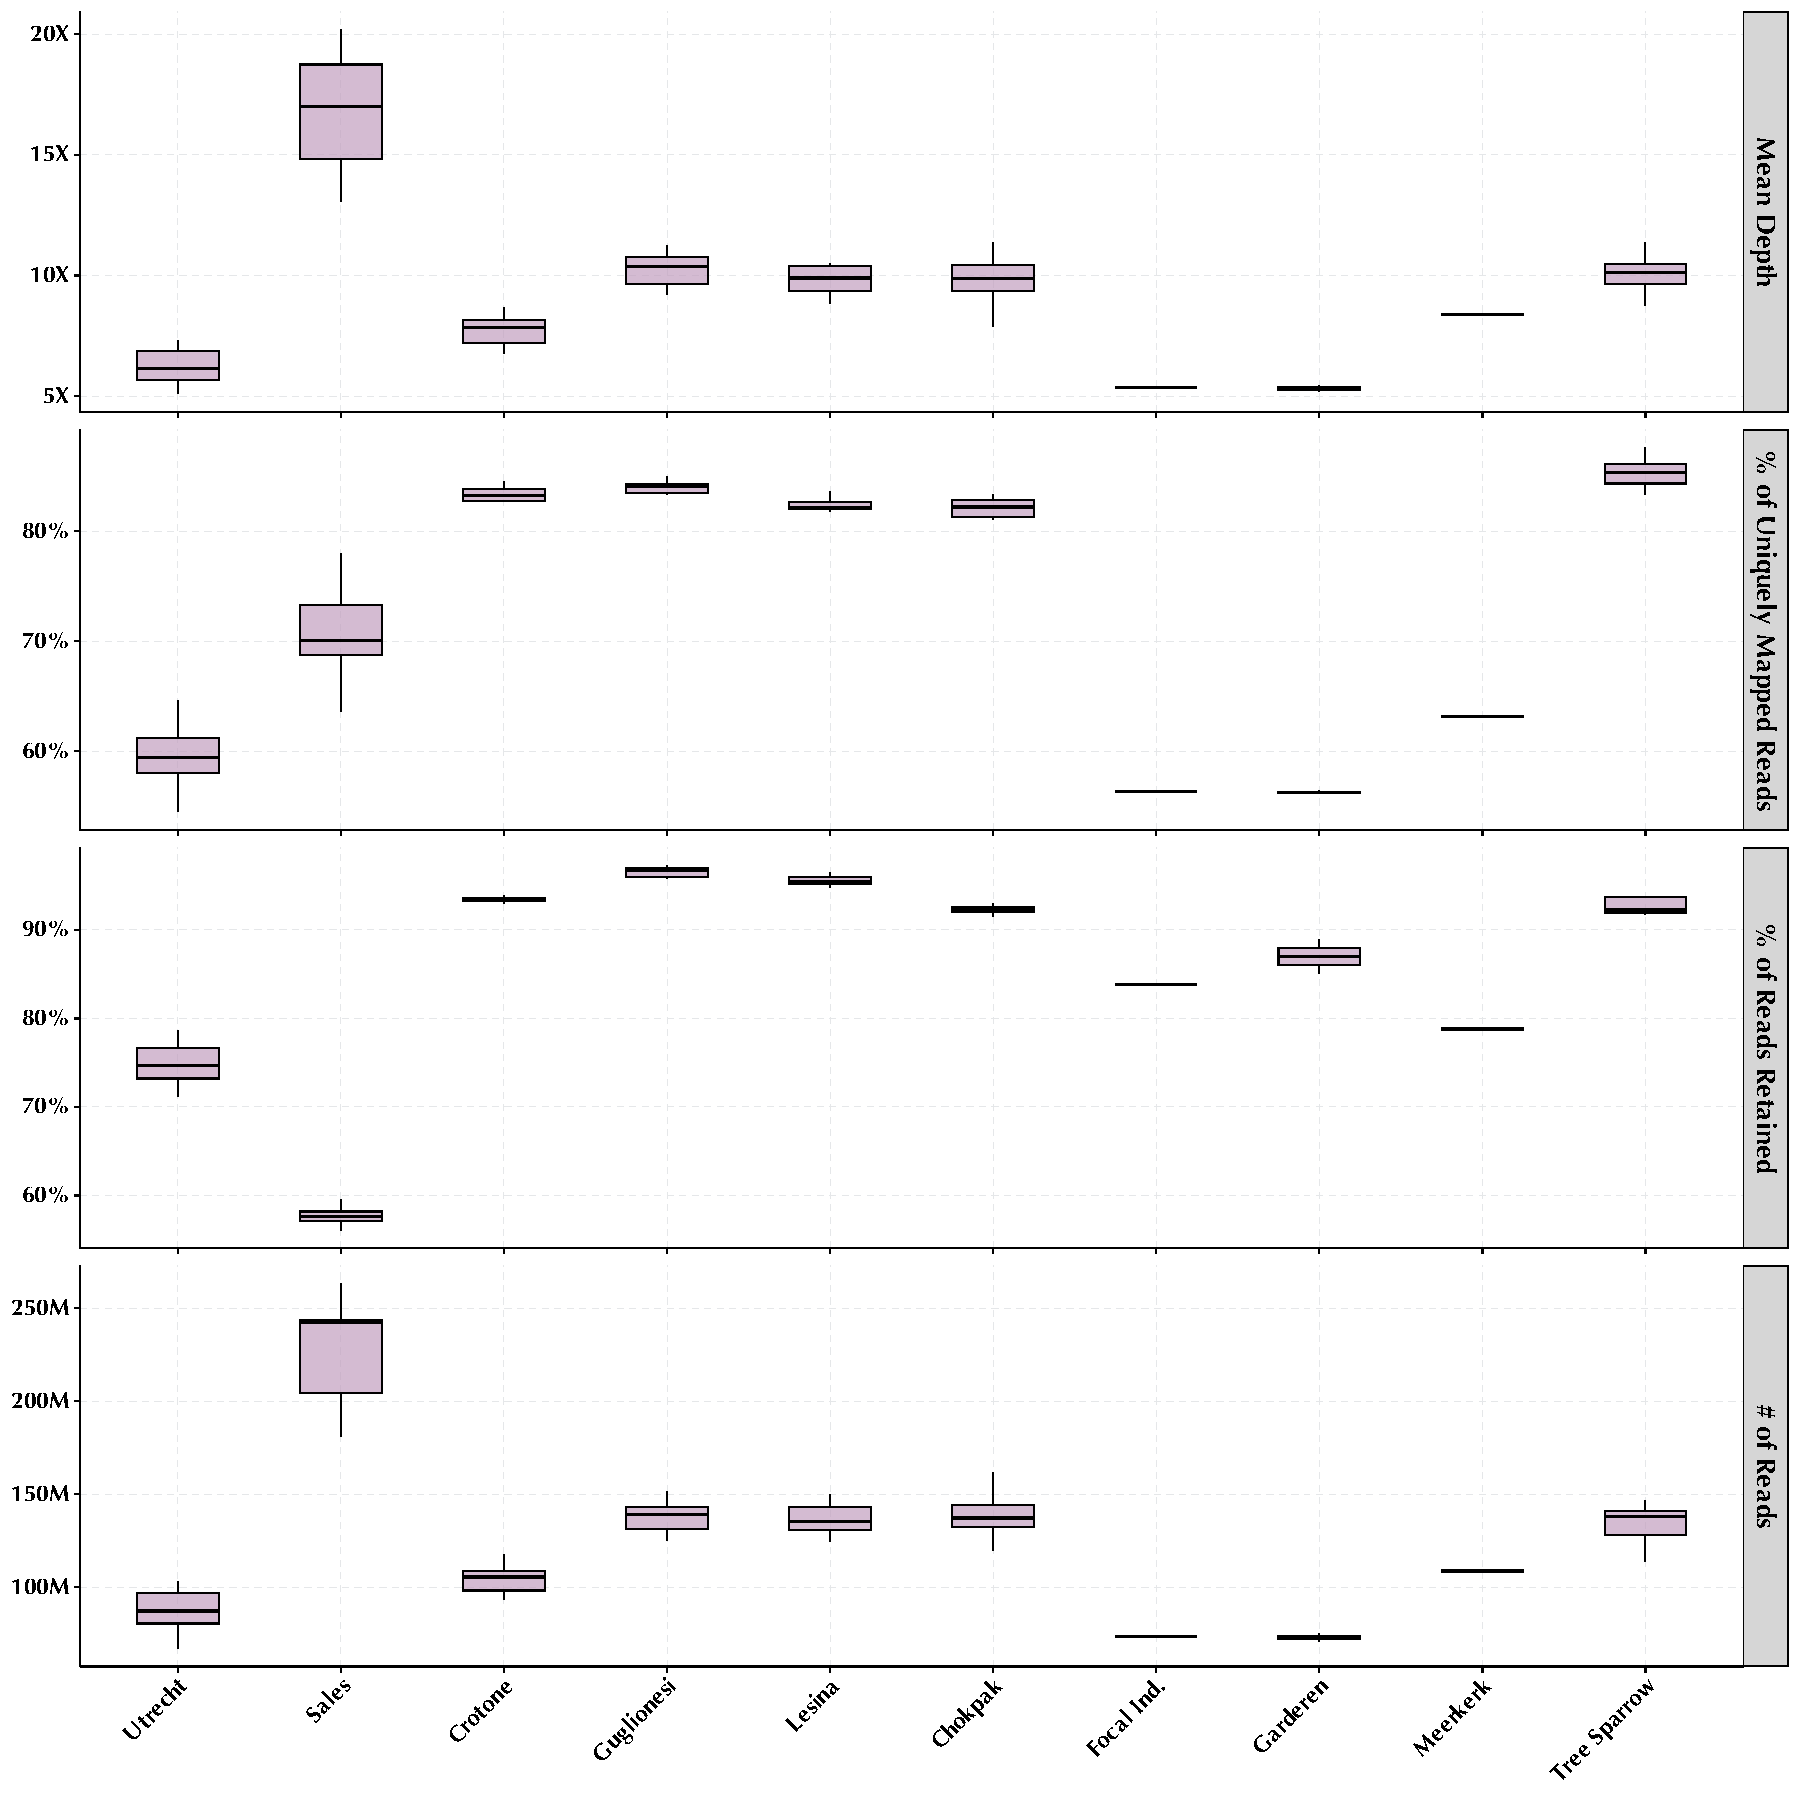
\includegraphics[width=\linewidth]{Figures/Y150239Genomics--Stats.pdf}
    \caption{Box plots summarising the processing and mapping statistics of the sequencing data analysed grouped by population.}
    \label{fig:SIfigure-01}
\end{figure}

\begin{figure}
    \centering
    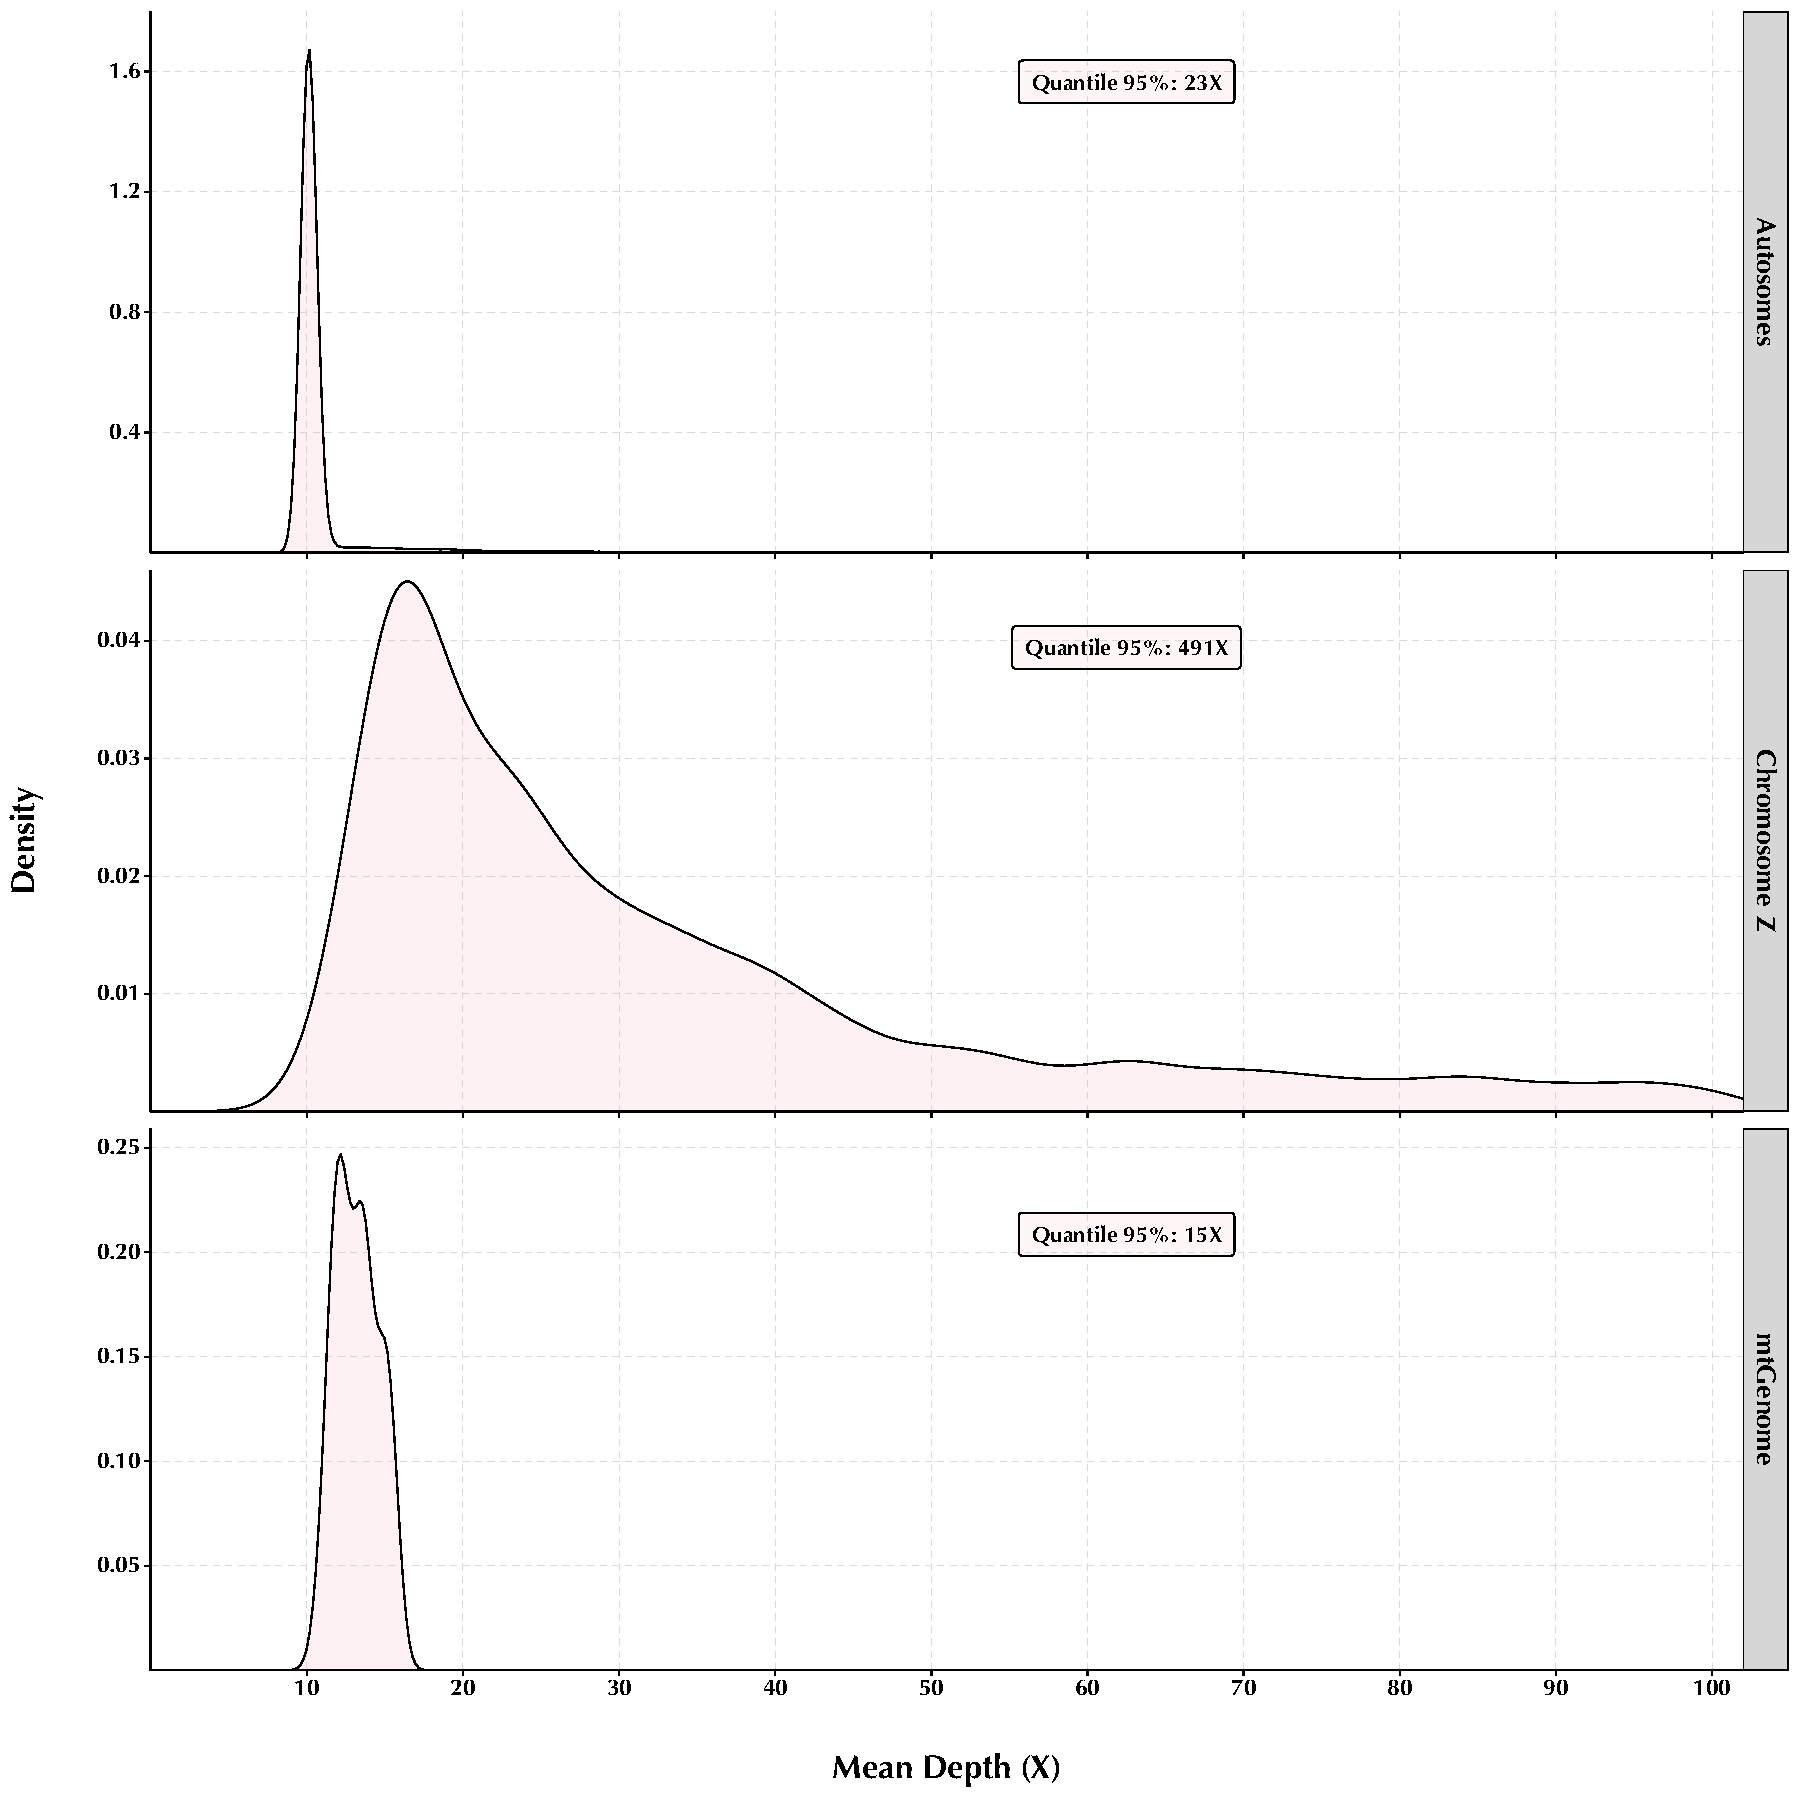
\includegraphics[width=\linewidth]{Figures/Y150239Genomics--MeanDepth.pdf}
    \caption{Density plots summarising the per SNP mean depth across all samples categorised by chromosome type.}
    \label{fig:SIfigure-02}
\end{figure}

\begin{figure}
    \centering
    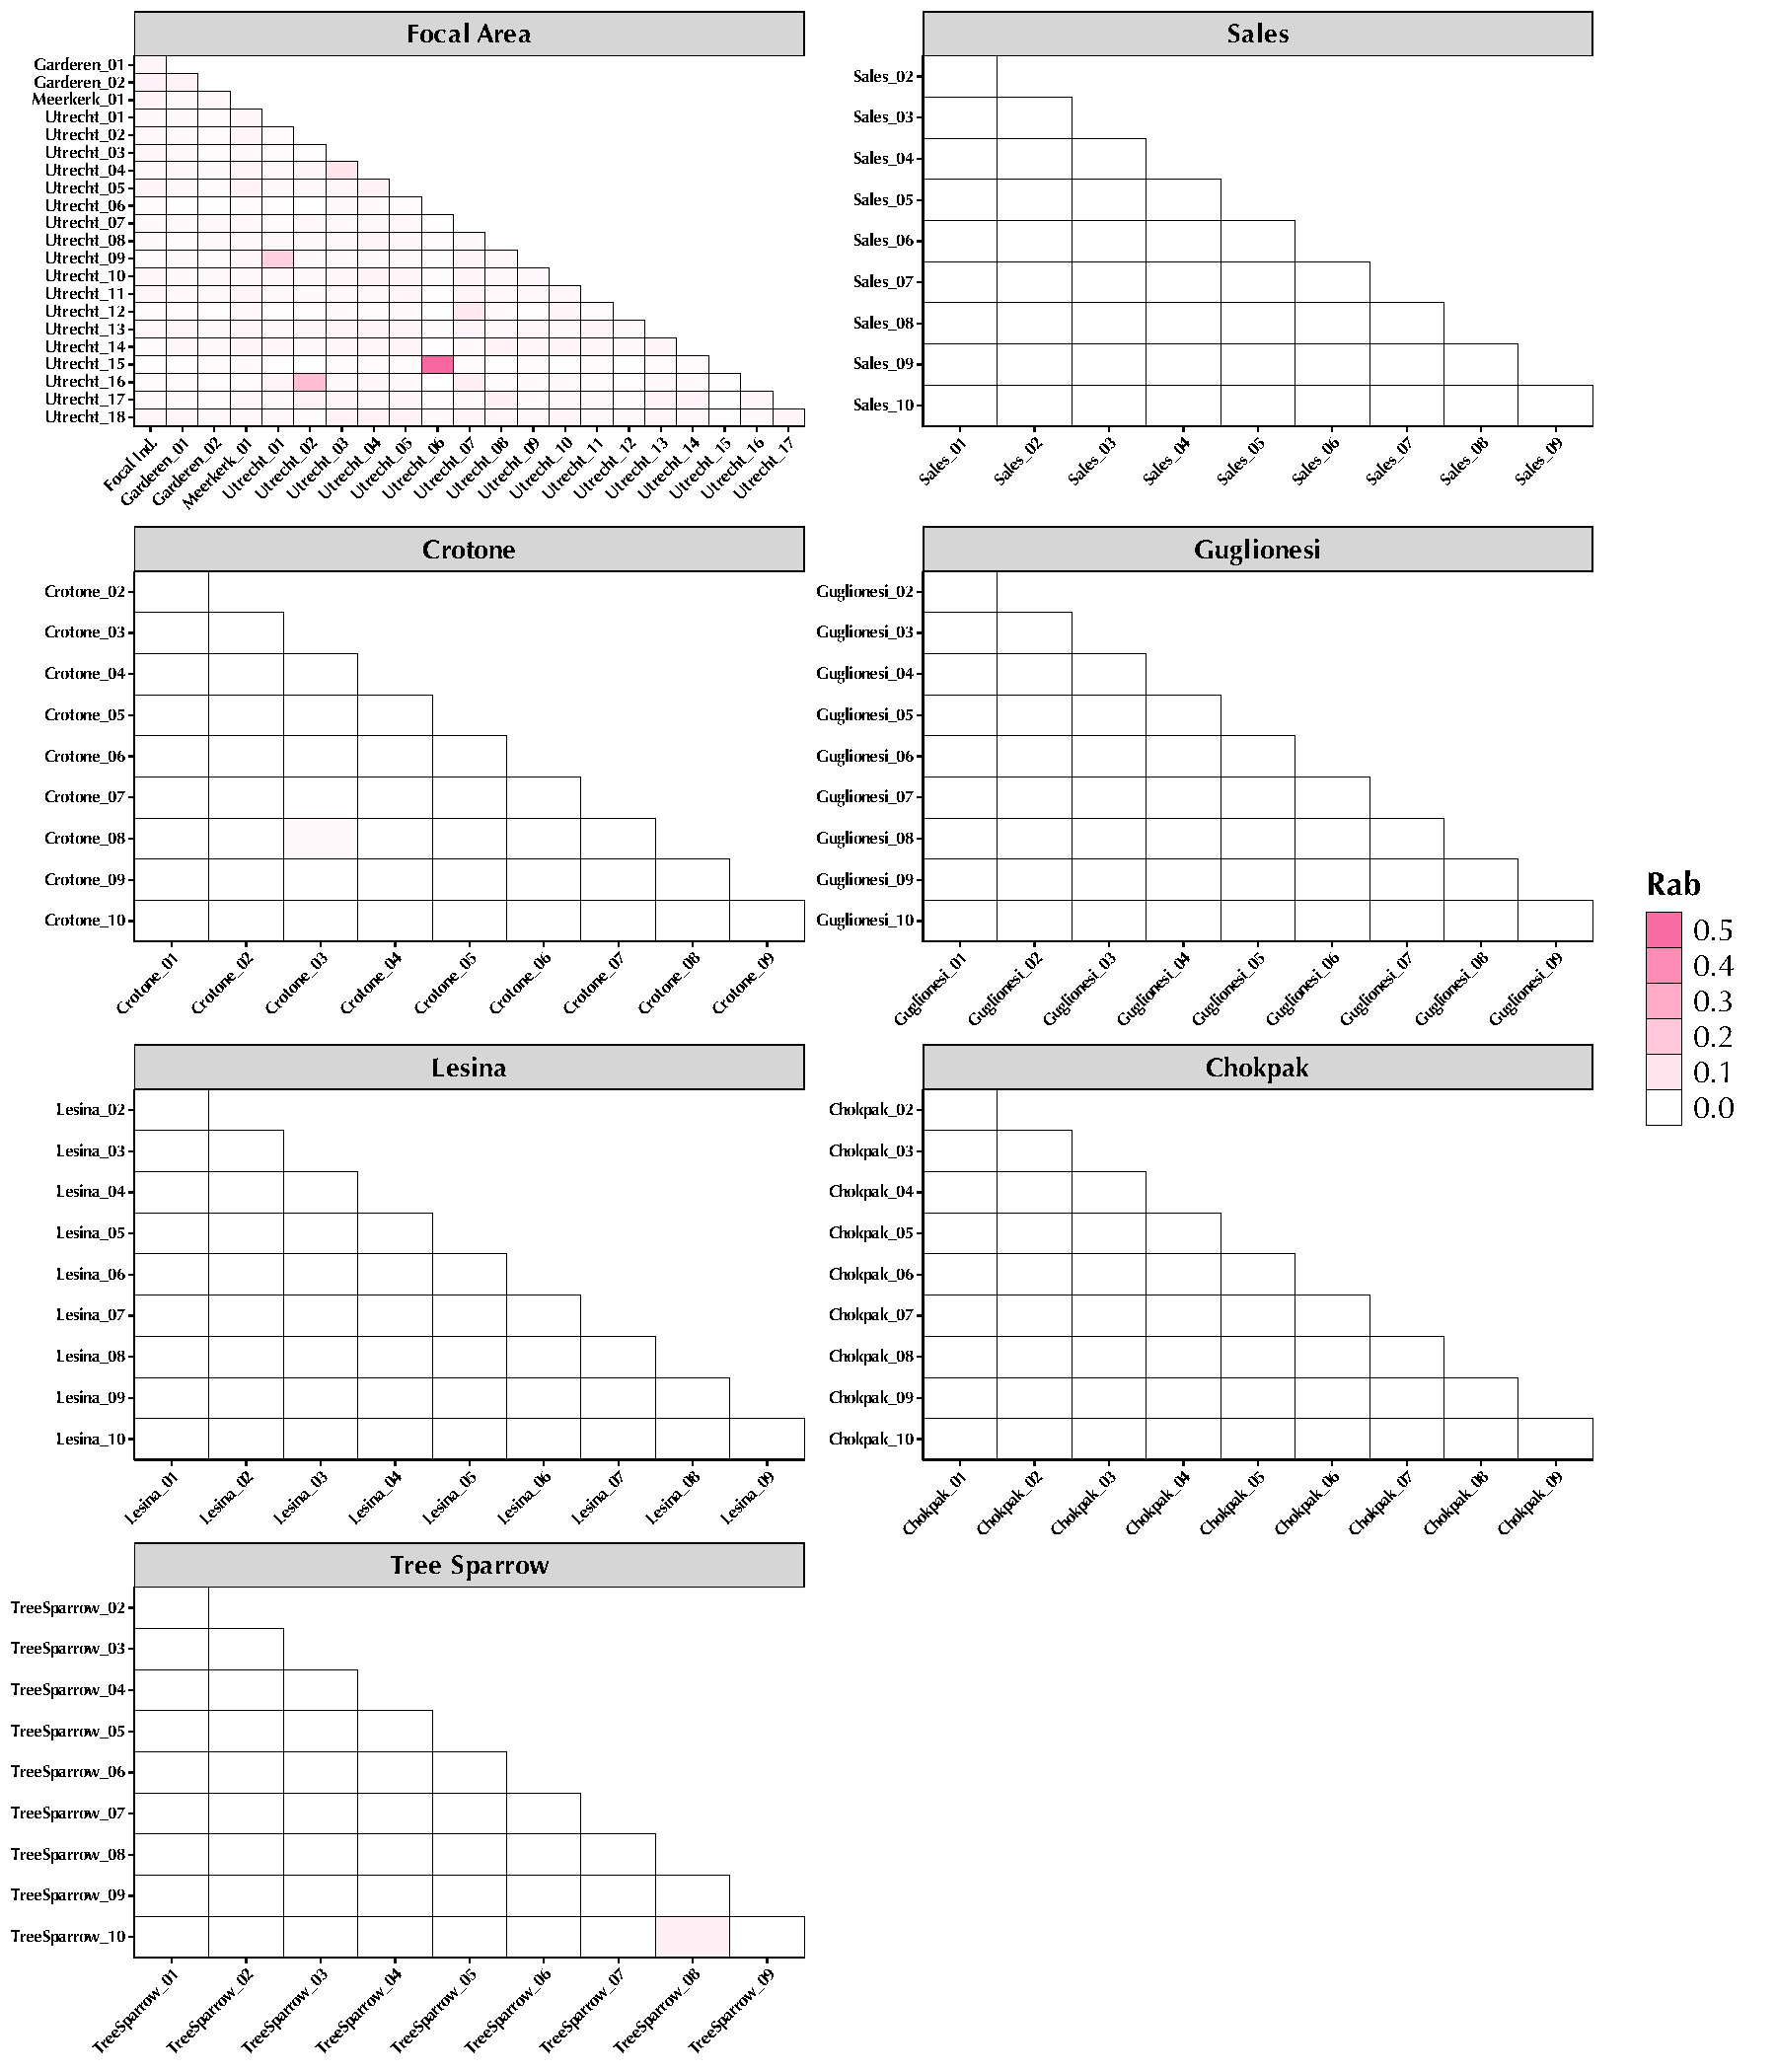
\includegraphics[width=\linewidth]{Figures/Y150239Genomics--Kinship.pdf}
    \caption{Heat maps of the RAB statistics based on the autosome genomic data grouped by population.}
    \label{fig:SIfigure-03}
\end{figure}

\begin{figure}
    \centering
    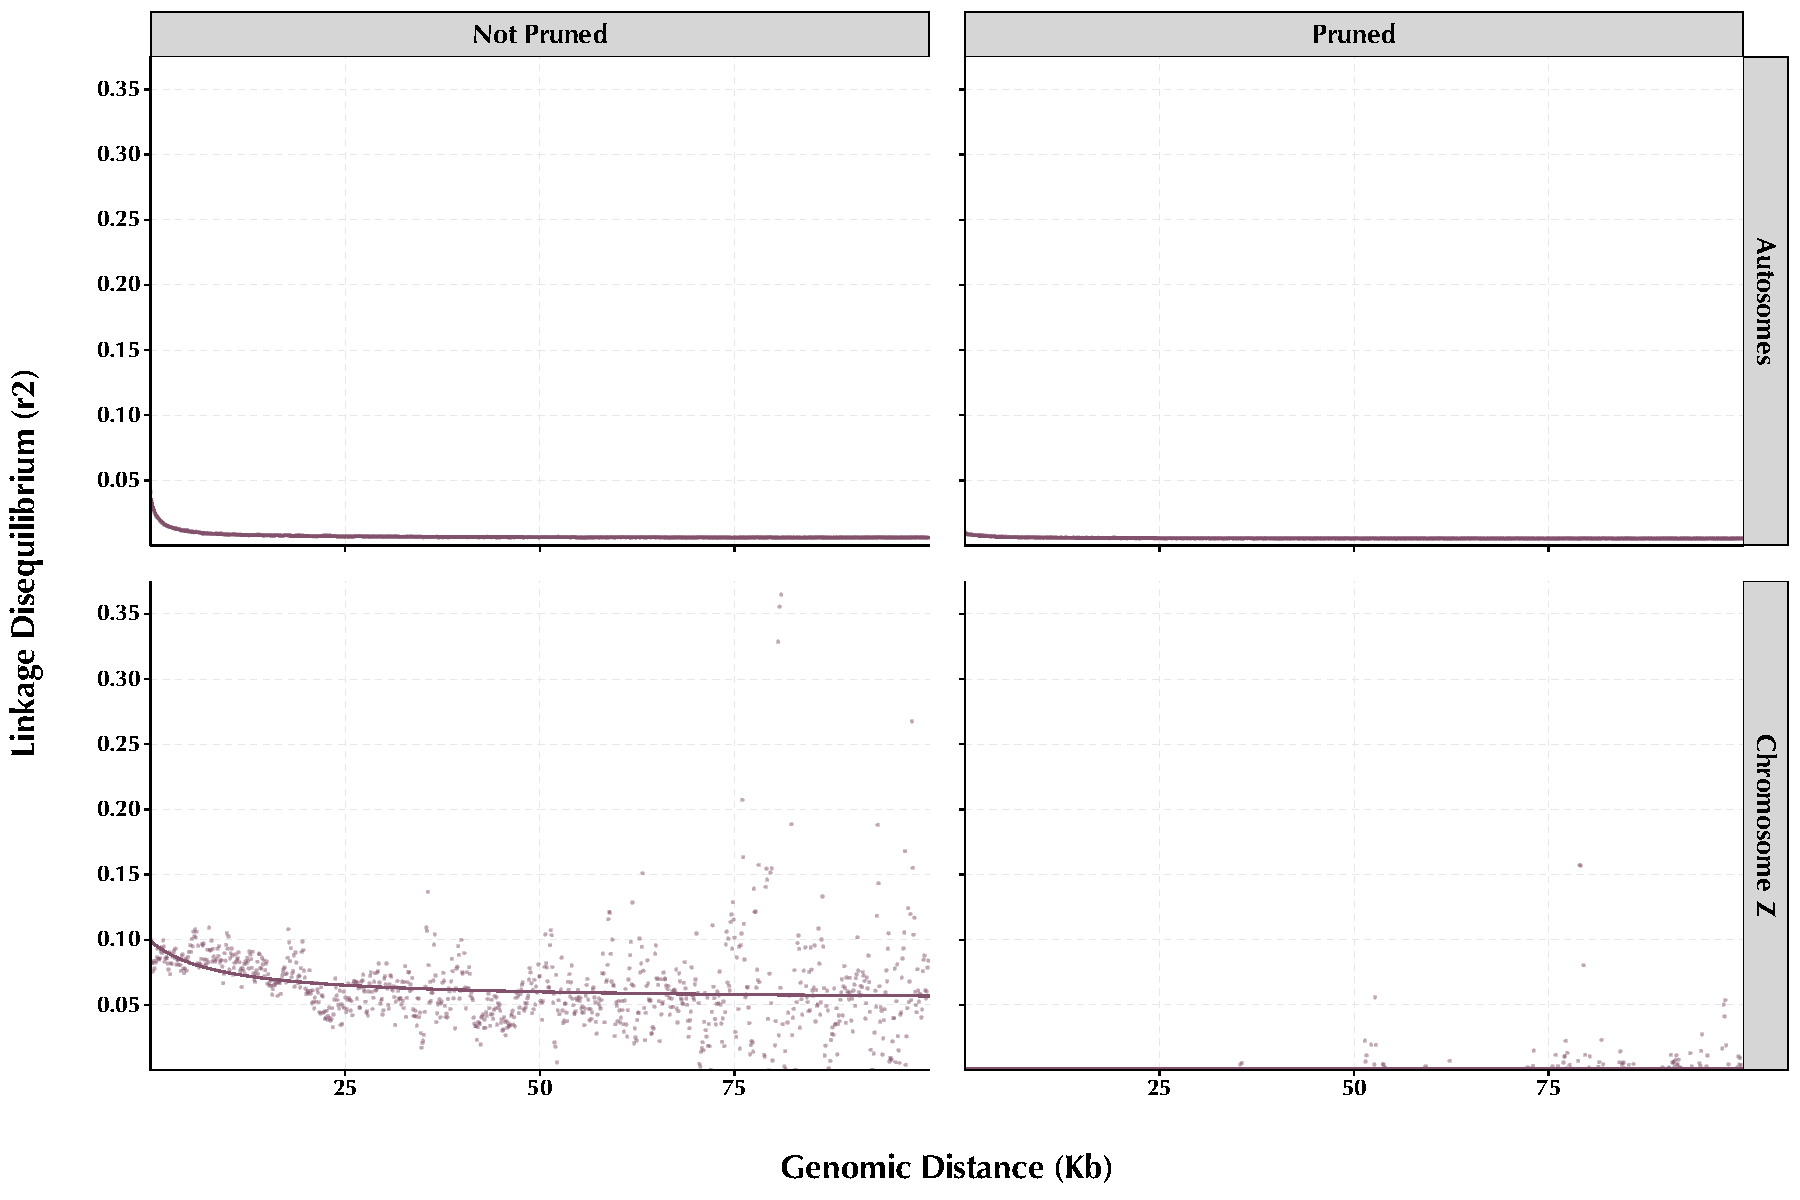
\includegraphics[width=\linewidth]{Figures/Y150239Genomics--LD.pdf}
    \caption{Linkage disequilibrium decays calculated individually based on chromosomal classification before and after linkage disequilibrium pruning.}
    \label{fig:SIfigure-04}
\end{figure}

\begin{figure}
    \centering
    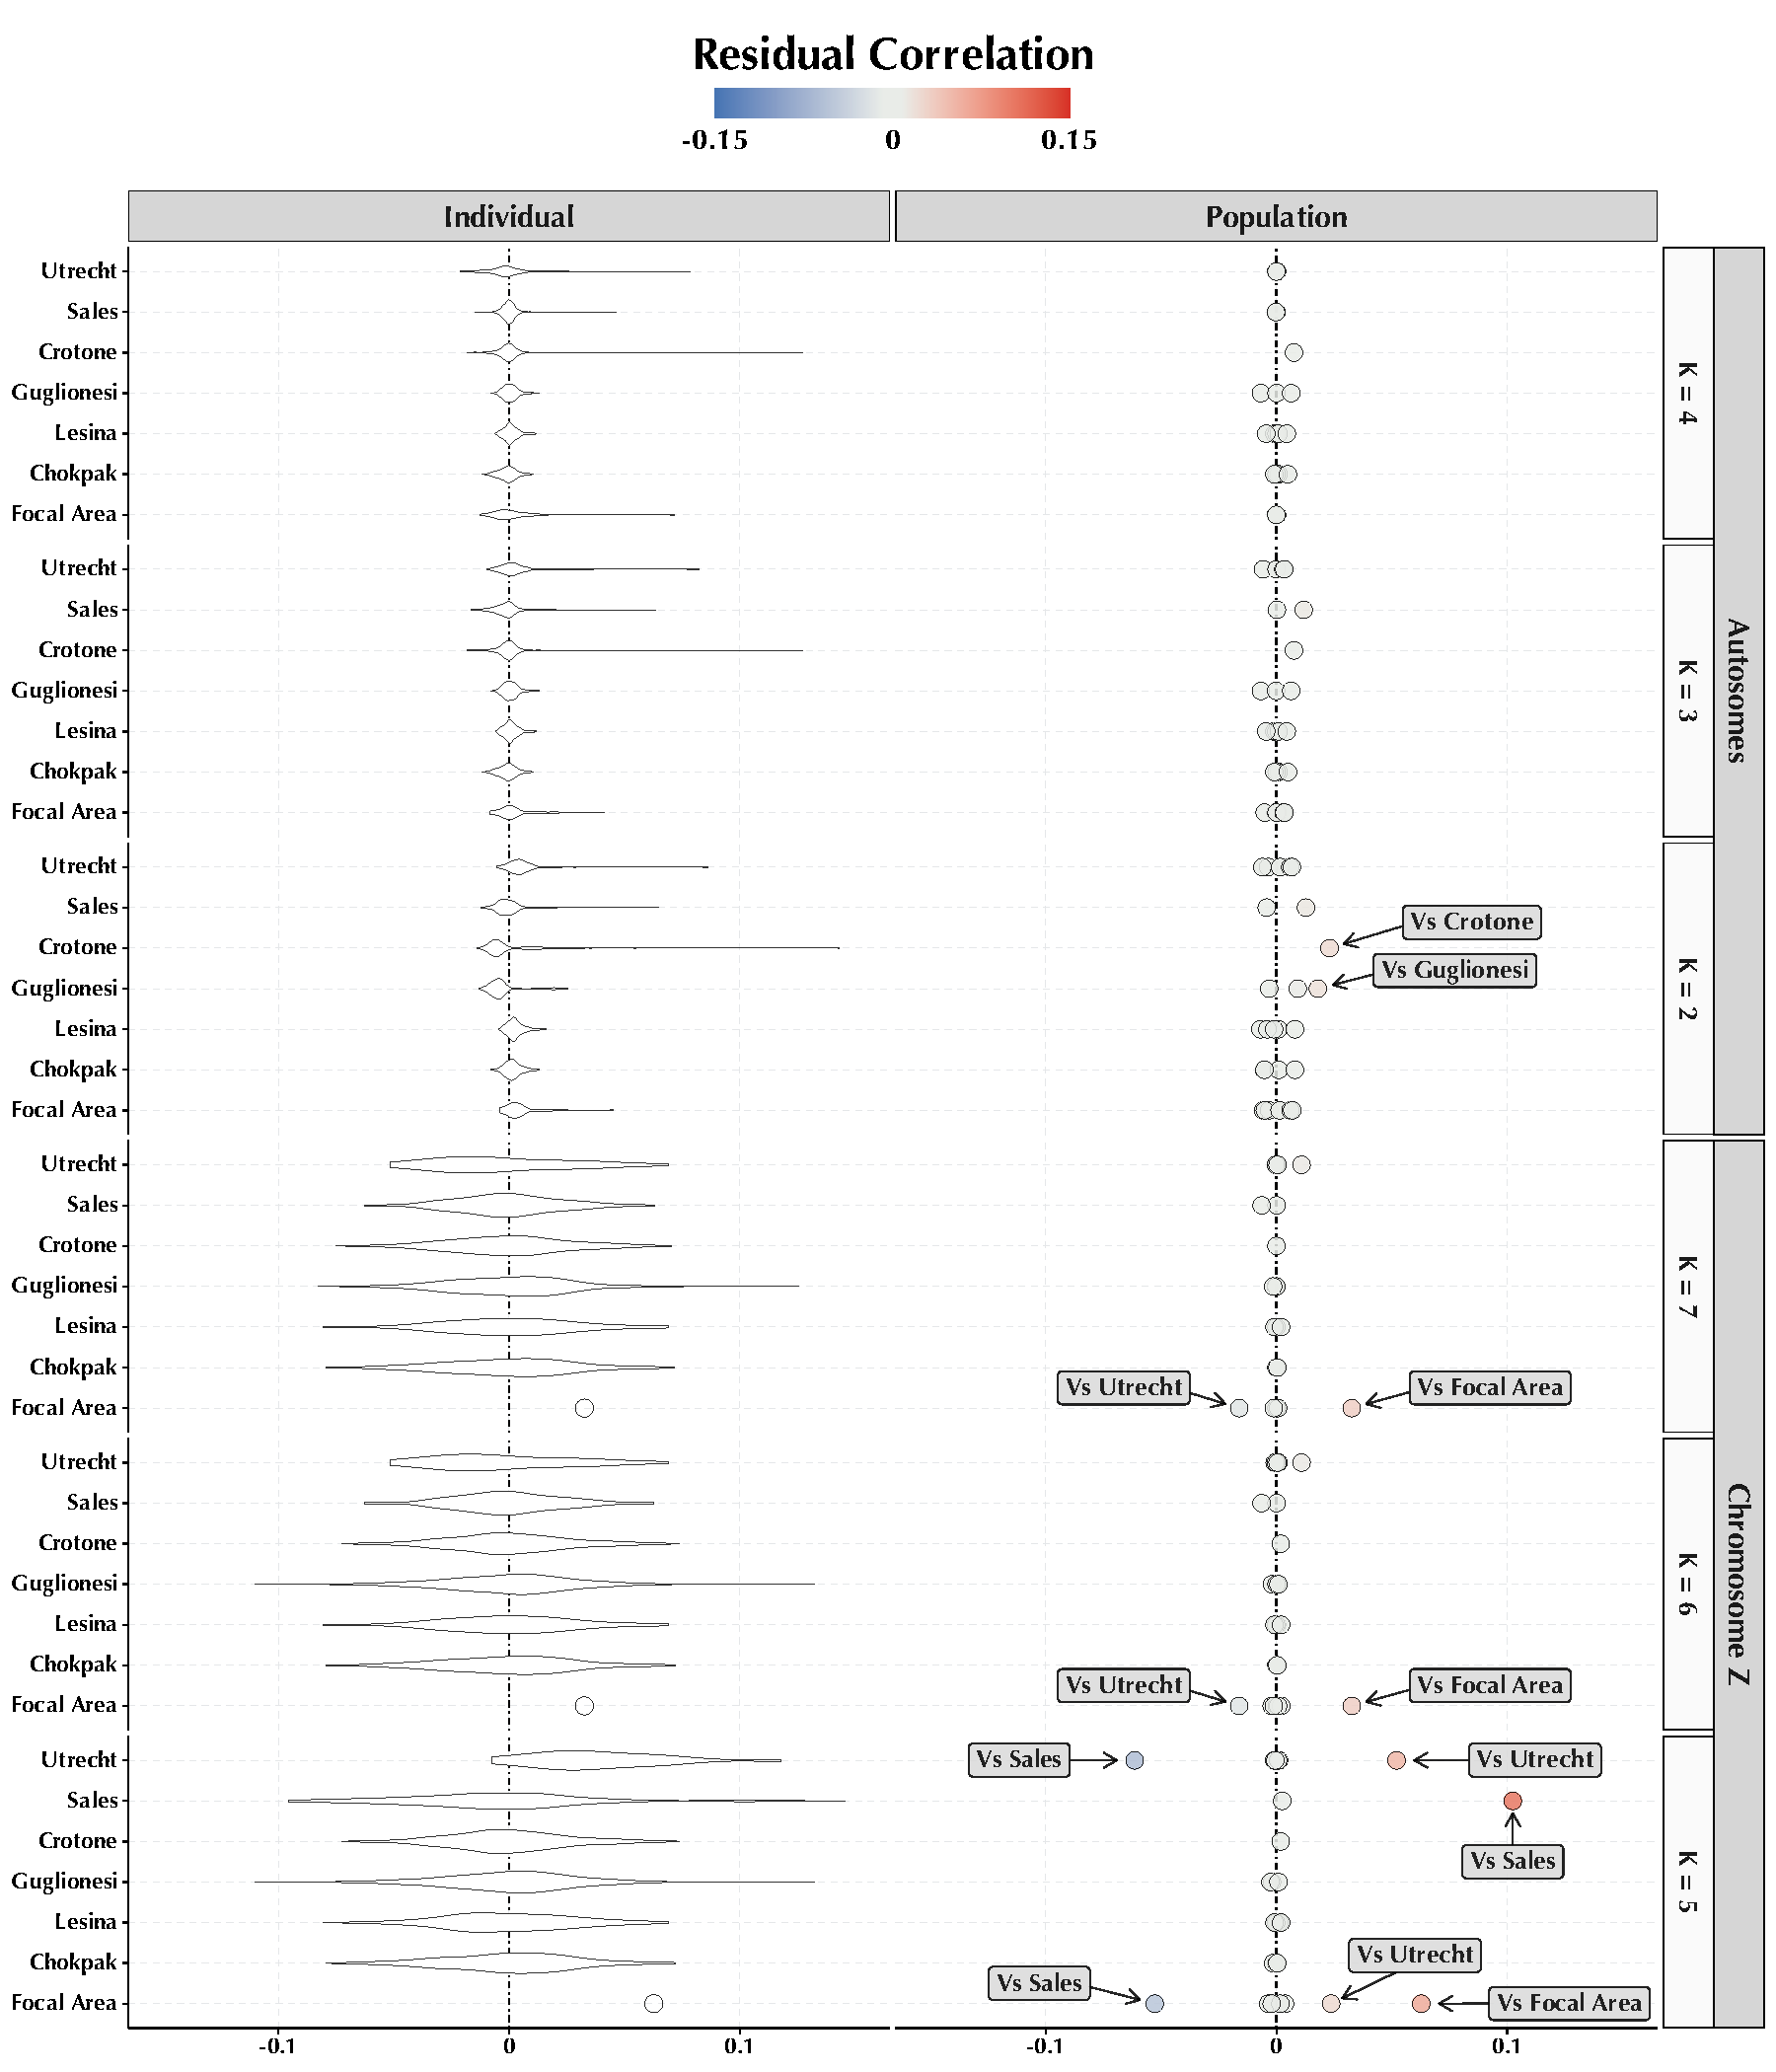
\includegraphics[width=\linewidth]{Figures/Y150239Genomics--evalAdmix_Points.pdf}
    \caption{Individual and population residual correlations for K = 2, K = 3 and K = 7 categorised by chromosome type and grouped sper population.}
    \label{fig:SIfigure-05}
\end{figure}

\begin{figure}
    \centering
    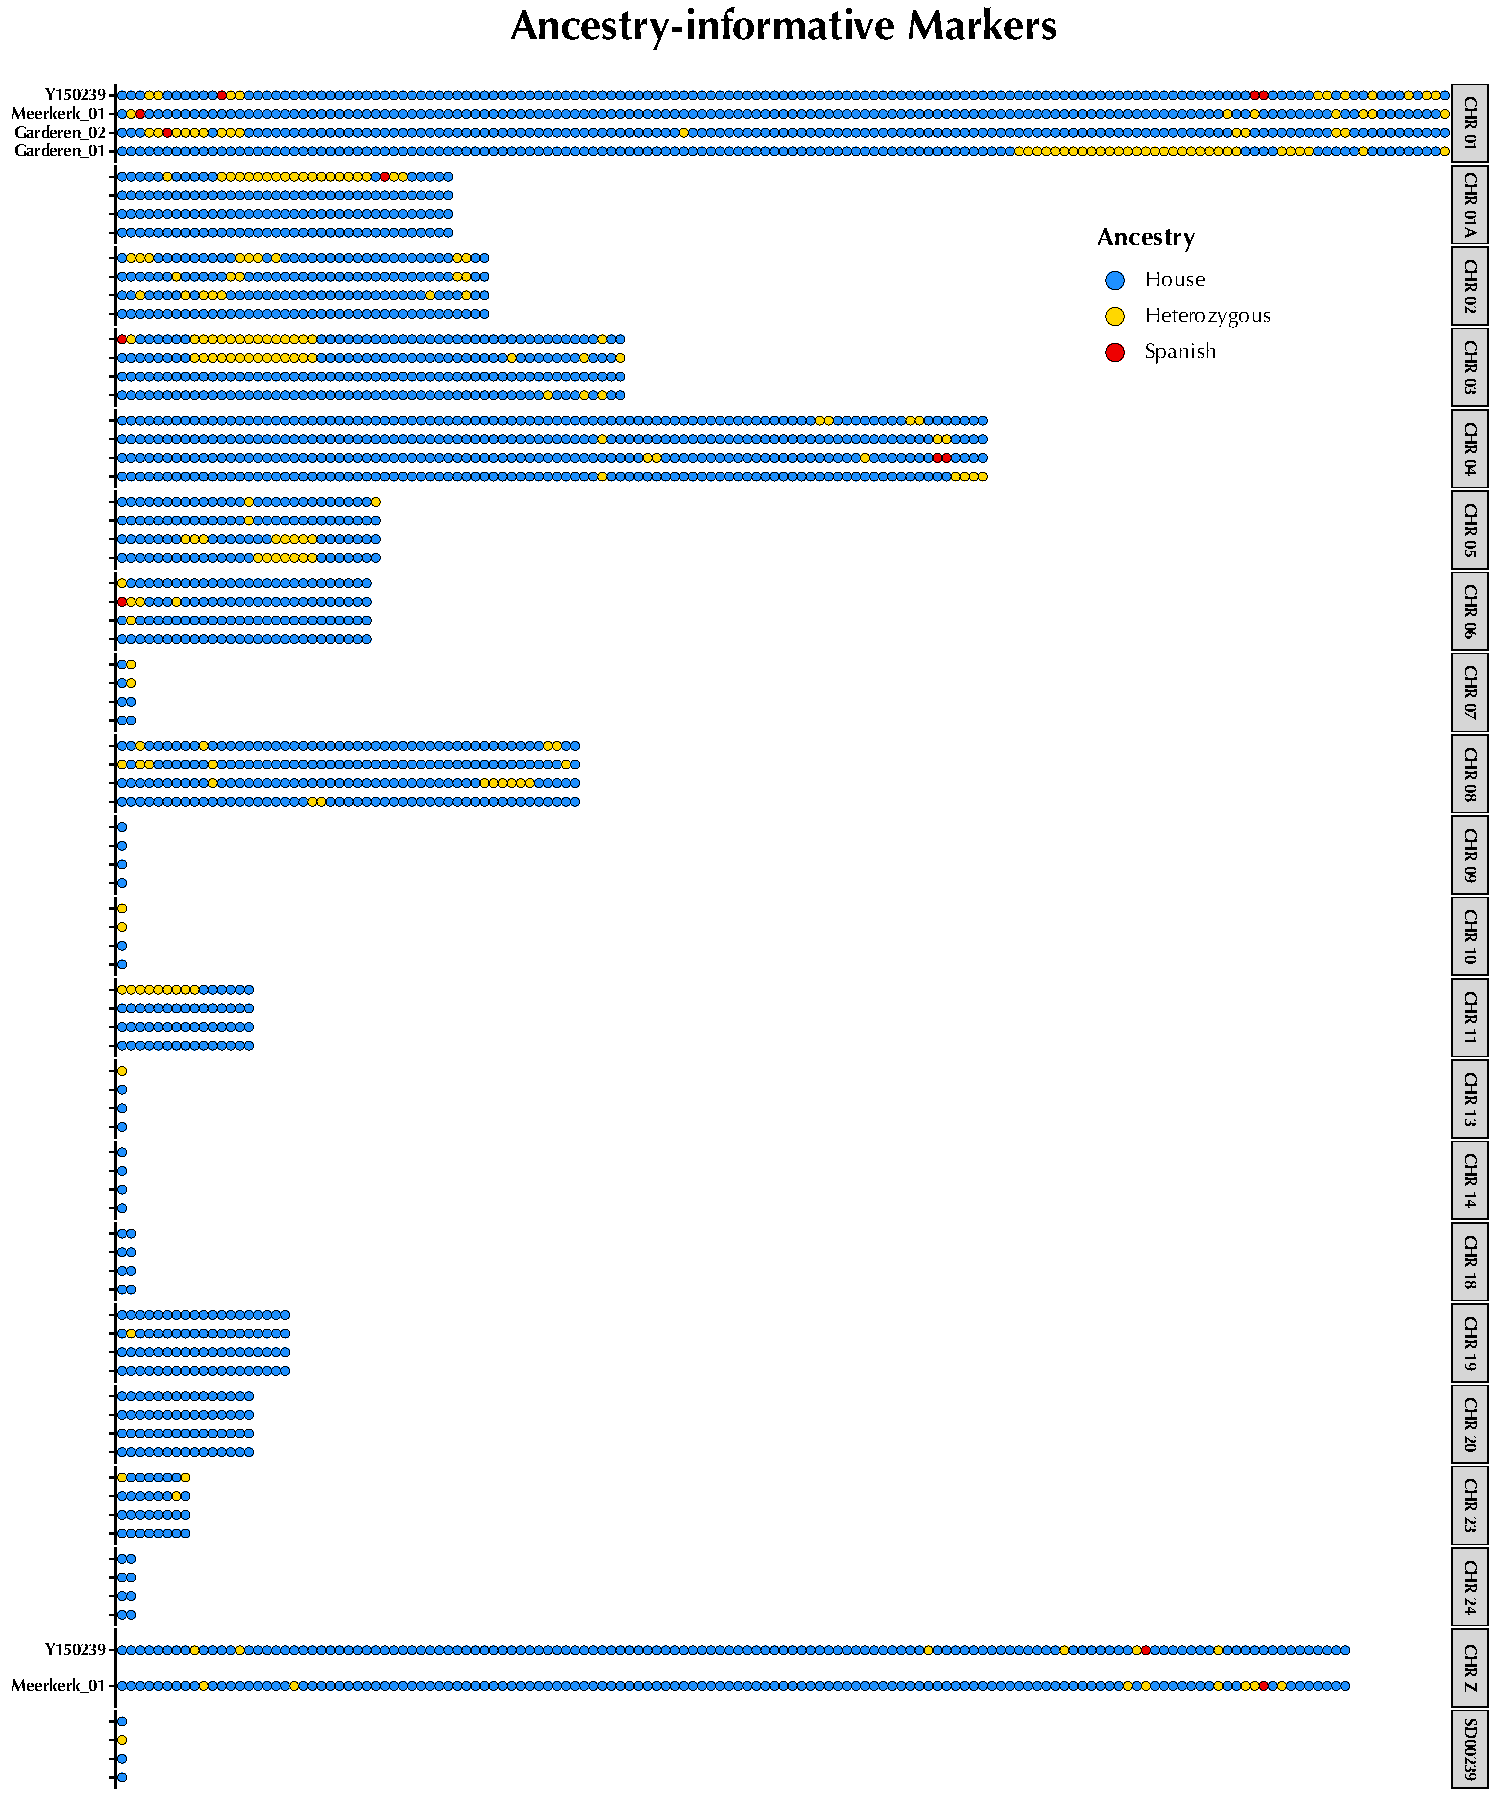
\includegraphics[width=\linewidth]{Figures/Y150239Genomics--AncestryHeatmap_AIMs.pdf}
    \caption{Genotype state of the ancestry-informative markers categorised by chromosome/scaffold for the four individuals within the focal area.}
    \label{fig:SIfigure-06}
\end{figure}